%\chapter{Further Installations}

\iffalse
\section{GRU Chatbot Coding Experiment}

We code our own version of the GRU model. We refer to the Inkawhich et al \cite{2018Inkawhich} tutorial frequently. For this code we use the Movie Dialog Corpus. This is the same corpus that the tutorial uses, and is the same corpus we used in the larger Transformer model chatbot.

The GRU coding experiment is considered unsuccessful. For all Raspberry Pi installations we use the GRU tutorial. % from Inkawhich. % et al \cite{2018Inkawhich}.

The major differences in the code from Inkawhich et al %\cite{2018Inkawhich} 
and our code for the GRU chatbot is that they use their own loss function while we use a Pytorch loss function. The loss function we use is called `CrossEntropyLoss'. Also they use Beam Search while we use an `argmax' function. An explanation of Beam Search is beyond the scope of this paper. The tutorial also uses the `Dot' attention while we use the `General' attention. 

Comparing these attention mechanisms you might consider the `Dot' attention to be the simplest, while the `General' attention is more complex. Most complex of the three methods considered would be `Concat' attention. These approaches are touched on in section \ref{section-gru-attention}.

Because of these differences the tutorial code trains to completion in under an hour on a cpu based machine. Our code trains for several hours before the kinds of replies that it gives are satisfactory.

\fi

\section{Generative Pre-Training 2 - XLarge Model}

The large 774M model of GPT2 was ultimately released to the public. In addition to this, two other models were created. One, named `x-large,' had 1.5 Billion parameters. Another, named `xx-large,' had 8.3 Billion parameters. We download the `x-large' model for testing purposes.

The tests from the previous sections worked on the `large' 774M model. Subjectively the answers provided by the 1.5B model were better. The answers were stronger grammatically.

The 1.5B model is too large for a Raspberry Pi, using 12.3 Gig of ram while it is running with inference. We experiment with the model on the development laptop computer.

As with the smaller model and the Raspberry Pi installation, we do not attempt transfer learning on the model. Instead we show the model specific information during inference which the model is free to reply with if it finds the information appropriate.

We also want the model to be able to summarize articles from the internet and reply with that information when asked to do so. 

\label{chapter-gpt2-xl-intro}

\subsection{Context Experiment}

As before we gave the model details in sentence form that it could use as reply to questions when appropriate. The larger model works better if all the sentences shown to it have the `Q:' and `A:' strings prepended to them. 

In each example the information we wanted the model to choose from was presented in sentence pairs. Though these sentences look much like source/target pairs from our movie corpus, they are totally unrelated.

An example might be the presentation to the model of the model's name. In the smaller GPT2 model we simply show the model the single sentence `My name is Jane'. In the larger GPT2 model's code we must show the model two sentences. One is `Q: What is your name?' and the other one, following it directly, is `A: My name is Jane'. We follow these conventions for the time of day, the model's location, and the model's occupation.

These sorts of questions can be answered without any memory of what the last question was.

\subsection{History Experiment}

We tried concatenating all input and output and including it with each question. While this did little or nothing during the smaller GPT2 experiment, with the larger models the history sentences were helpful. Consider the questions below.
\begin{verbatim}
> Do you like the color red?
I like the color red.
> What is your favorite color?
Red.
\end{verbatim}
This is the same text excerpt as from the small GPT2 model in Section \ref{install-gpt2-history}. The `favorite color' example continues to work on the larger GPT2 model. Again as in the small model, the chatbot is keeping track of the conversation. 

Even though the history is consulted before answers are formulated, the output of the model is not always predictable. This has something to do with the `temperature' setting of the model. The output is sometimes more fanciful.


\subsection{Artificial Intelligence Markup Language Experiment}

We want to be able to tell the model exactly how to answer a given question if we have a particular need. For example, the GPT2 models that we have handle remembering the user's name very badly. We would like to dictate how the model handles that situation. We have employed Artificial Intelligence Markup Language for this. 

AIML is actually poorly suited for handling this task. In AIML you must code every question and response as a separate rule. If you have a question `How are you?' and an answer `I am fine' the AIML kernel will only answer with the programmed response if the input is an exact match. If you enter `How are you doing?' or `How do you feel?' the kernel does not have an answer for that. The two or three questions are phrased differently but can be answered with the same text.

The GPT2 chatbot is much different. Groups of questions have the same answer. Sometimes the answer could even be `I don't know', but still the answer makes sense in English. The chatbot could answer `How are you?', `How are you doing?' and `How do you feel' with one answer like `I don't know' or `I am fine'. These questions are phrased differently with the same answer.

For us to use AIML for our task we code questions and answers in pairs for all possible phrasing of a question.

We have to count the number of AIML rules that we are coding and compare it to the number of English sentences that the GPT2 chatbot can answer. We have to make sure that the number of chatbot answers is much higher. As it stands the number of GPT2 chatbot answers dwarf the AIML rules.

We prefer the answers provided by the generative chatbot over those provided by an AIML file. We want to maximize the amount of time that the overall model answers using the Transformer that is internal to the chatbot, and minimize the use of AIML and the AIML kernel. We set a criteria for ourselves. If the generative chatbot is handling most of the questions and answers then we can proceed. If the AIML question/answering set is larger than the number of questions that the chatbot can answer, then the AIML should be avoided. 

Below we illustrate two situations where AIML might be useful. In both cases the AIML files are small.

\subsection{User Name Experiment}
The name of the user is our first example of AIML coding. This example is easy. There are few ways to say `My name is *'. In this case `*' is a wildcard. Another variant is `* is my name'. That's as many ways to say it as there are.

Each question is answerable with a phrase like `Hello *'. Here the asterisk is a wildcard for the memorized name. An AIML file can handle this sort of question very easily. We write an AIML file with these questions. We depend on the AIML to remember the name from the wildcard. 

Another question in this scenario is `What is my name?' With this question also there are very few ways to phrase the AIML. Here we are referring to the name recorded in the previous AIML question as discussed above. 

During a typical chatbot run we show all user input to the AIML kernel. 

When the kernel does not match anything there is no output from the kernel, but when there is a match we show the AIML output to the chatbot as the context for that input. This is to say that the input from the user is concatenated with the context text, in this case the answer from the AIML kernel. The chatbot is then left to decide what to answer from the user question and the context. Usually the answer makes sense.

Usually the user's question and whatever the chatbot decides will be the answer are both added to the history. As noted before, history of what the user enters and the chatbot's answer are kept by the chatbot so that the chatbot can keep track of answers over time. Sometimes, though, keeping sentences that refer to user names confuses the bot's answers. In other cases the bot keeps track of answers that are generated in the AIML/chatbot hybrid process.

Even when the answer makes sense there is only a certain percentage of time that this example works. Sometimes, even with the coaching of the AIML, the model does not answer with the right name. Sometimes you ask it for your name and it responds with it's name. Some times you ask it for it's name and it responds with yours. Without the AIML the model always answers all name questions with it's name. 

We suspect if the model was much larger that it would have less trouble with this kind of example.

\subsubsection{Usage Example}

The user might say `Hello, my name is John.' The bot might reply `Hello.' The user might then say `What is your name?' The bot should reply `My name is Jane.'

Then the user might say `What is my name?'. The bot should reply `John.'

In practice the bot will reply with `Jane' most of the time without the AIML augmentation. With the smaller GPT2 model the reply is often `Jane' even with the AIML kernel. With the larger GPT2 model the bot tends to answer what the AIML suggests for its answer. In this case the answer would be `John.'

\subsection{Internet Search Experiment}

We want to be able to search the internet for an article, download that article, and summarize parts of the article as answers to questions asked of the model. This is leveraging of the token size of the input to the model. It's usually very large. It can be 1280 tokens.

The AIML required is minimal but larger than the AIML for the `user name' problem. The goal is to detect when the user wants to talk about an internet page and detect when they are done.

The first case, when the user wants to talk about an internet page, is associated with utterances like `Tell me about *' and `I want to talk about *' where `*' is a wildcard for what the user is interested in. There can be other phrases that imply the same intention on the part of the user. In these cases the text from the wildcard in the invocation is saved.

The second case, when the user is done with the internet page and wants to return to normal operation, is associated with utterances like `Ok thanks' and `That's enough'. These two phrases can be checked for when the bot is in `Internet-Search' mode. There could easily be other phrases that cause the same operation in the chatbot code.

When the AIML detects one of these signals the program goes into a special mode of operation. The first signal, we will call the `find' signal, causes operation of an internet browser. The web search uses the text from the invocation of the `find' command. The browser yields results as they would be found using a google search engine. The first 20 results are kept and the url for the highest ranking wikipedia page is retained. That page is loaded and the `body' tag is scanned for `paragraph' type content. This web page replaces the context input. 

After that the context is retained while the chatbot answers any questions that the user might have. The GPT2 model has some facility with this, and the larger GPT2 model is more adept.

Later when the AIML detects the second signal, we will call the `restore' signal, the program switches back from special operation to normal operation. The web page contents are removed and the context is restored as it was during regular chatbot use. There is a part that has the history of the last few questions and answers, and there is a part that has the bot name, occupation, and the current time.

As the chatbot answers questions the content of the conversation is saved for the `history' of the context text, as it is used in the regular chatbot mode. This means there is a record of the questions and answers the chatbot goes through during it's operation, even when it is answering questions about a web page that it has searched for. Because of size limitations the history is not included in the chatbot input when it is answering questions about a web page, but a record is kept of `q' and `a' and the bot can refer to them later.

Again, because of size restrictions there is no regular context information shown to the chatbot while it is answering questions about a web page. Then, after the `restore' signal, the chatbot sees only the regular context and none of the web page material. The regular input for the small model is 768 tokens and it is more than 1000 for the larger models. Though this would appear to be a large space for text, it is common for wiki articles to be clipped so that the user's question can be inserted at the end.

\subsubsection{Usage Example}

Consider that you are interested in the musical group `The Beatles'. If you wanted to find out about the band you might say to the chatbot `Tell me about the beatles.'

The chatbot would take a little time to respond. During this pause the model is downloading an article from Wikipedia. Ultimately it would answer with something like `The Beatles were an English rock band formed in Liverpool in 1960.'

Then you might ask it a question like `How many members were in the band?'

To this question the 774M chatbot answered this way for us, `The Beatles were originally formed by John Lennon and Paul McCartney in Liverpool.' We note that this is not actually the correct answer. This may be because after clipping the information asked for does not exist in the context section. You can ask other questions. Some of them may be answered correctly and some not. 

To this question the x-large model answers `There were 4 members in the band.'

When you ask the question `How many members were in the band?' you do not need to specify which band. The model seems to be able to intuit the band that you are referring to.

At some point you will want to end the Q/A session. You would say `OK' or `OK thanks'. After that the web page for the `Beatles' would no longer be available to the chatbot. It could still answer questions. You could ask `What are the Beatles'. You might get an answer like above, `The Beatles were an English rock band formed in Liverpool in 1960,' even though the wiki page is not available to the bot.

This is an example of using the model. Other topics can be asked about. You do not need to re-start the model to ask about a second or third topic. On a CPU each question takes several seconds before an answer is produced. The large version of this model does not work on the Raspberry Pi.

If you use a GPU for your matrix multiplication the reply from the model would be faster. It might be instantaneous. On the smart phone and tablet Google has a product called the `Google Assistant'. The internal workings of the Google Assistant are not known, but if you ask it `Tell me about the beatles' the Assistant answers `According to Wikipedia the Beatles were an English rock band formed in Liverpool in 1960.' This is an answer culled from the same Wikipedia article that we use in our example above. The Google Assistant could use a Transformer architecture internally.

\label{chapter-xlarge}

\section{Generative Pre-Training 2 - Jetson Nano}

\label{chapter-nano}
The NVIDIA Jetson Nano is a small single board computer that has a GPU and runs on the aarch64 platform. It has 4 Gigabytes of ram.

The Jetson Nano was used as a platform for the GPT2 117 Million parameter model. The Nano uses an NVIDIA GPU. Initial tests showed a model that could answer a basic question in two to three seconds. Previously a Raspberry Pi computer would take approximately thirteen or fourteen seconds. On the host laptop, where development was done, the 117M model still outperforms the Nano. On the host laptop the model replies to a general question in around one second.

This smaller 117 million parameter model was not used for the sort of Wikipedia searches that were attempted in Section \ref{chapter-gpt2-xl-intro}. Instead it was used for the same basic chatbot task that was tested on the Raspberry Pi platforms.

Some details from this experiment are identical to Section \ref{install-gpt2-chatbot} or Section \ref{install-gpt2-smart} where the 117M model is installed on a Raspberry Pi.

The Nano that the GPT2 model was installed on was outfitted with a speaker, a microphone, and a wifi dongle. Pytorch for the Nano is installed from a community web site where version 1.5 or 1.6 was already cross compiled for the aarch64 environment. 

Response time with the Nano was reduced to just a few seconds. Response time on the Raspberry Pi for the 117M model was closer to 14 seconds. See the discussion of `Reply Time' in Section \ref{setup-reply-time}.

\begin{figure}[H]
	\begin{center}
		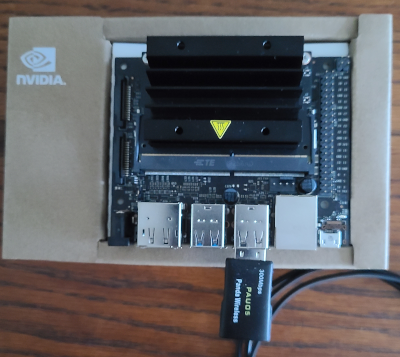
\includegraphics[scale=0.9]{diagram-jetson-nano-02}
		
		
	\end{center}
	\caption[Jetson Nano]{Jetson Nano without case.}
	
	
\end{figure}